% Provenance (never printed): see sources/outline_sources.md (Year 2: palaeogeography through
% the Phanerozoic; sea level; orogenies; mass extinctions and their Earth causes). Maps from the
% plate model of Merdith and others (2021) through the GPlates Web Service; sea level from the
% Miller and others (2005) NOAA study (Haq and others 1987; Kominz and others 2008); flooding and
% the Pitman model after Tasistro-Hart and Macdonald (2023); the big five after Marshall (2023)
% and Kaiho (2022); oceanic anoxic events after Rigo and others (2024) and Walker-Trivett and
% others (2024); CAMP carbon dioxide after Capriolo and others (2020); Chicxulub after
% Pickersgill and others (2026) and Collins and others (2020). Curves and numbers from
% figdata/bachelor-2/phanerozoic.py; exercise and problem values in the Book 4 scratch
% calculator calc/ch19.py.
\chapter{الأرض في دهر الحياة الظاهرة}\label{ch:b2:phanerozoic-earth}

في غرب كانساس، في وسط أمريكا الشمالية، تنتصب أعمدة من الطباشير الأبيض فوق
البراري. والطباشير هو وحل قاع بحر: فقبل نحو 80 مليون سنة كان بحر
ضحل يمتدّ من الشمال إلى الجنوب عبر وسط أمريكا الشمالية، وكانت أصداف
الطحالب الطافية تستقرّ على قاعه بمعدّل بضعة أجزاء من مئة من المليمتر في السنة. وخمس مرّات في
آخر 540 مليون سنة اختفت حصّة كبيرة من الأنواع الحيّة في بحار كهذه في غضون
لحظة جيولوجية. والقصّتان كلتاهما من صنع الأرض نفسها: فقد تحرّكت القارّات وارتفع البحر وانخفض فوقها،
ووقعت ثلاثة على الأقلّ من الانقراضات الخمسة الكبرى مع تدفّقات حمم من باطن
الكوكب. يتتبّع هذا الفصل دهر الحياة الظاهرة عبر خرائطه، ومستوى بحره، وأحزمته
الجبلية وأزماته، ويضع أرقامًا على اثنين منها: بأيّ سرعة ترفع الظهرات البحر، وكم من
اليابسة يُغرق بحر أعلى.
% ledger: kgs:monument-rocks, kgs:chalk, ics:base.Phanerozoic, kaiho22:table, cr03:table

\begin{recall}
\textbf{من مجلدات المدرسة}: تكتونية الصفائح وبانجيا؛ والأحافير والسلّم الزمني
الجيولوجي؛ والتجاوزات البحرية مقروءة في جرف. \textbf{من مجلد السنة الأولى}: قانون العمق--العمر
لقاع المحيط؛ والمنحنى الهيبسومتري؛ والتوازن الأيزوستاتي؛ والسكونية ومستوى البحر النسبي؛ والمقاطعات
البركانية الكبرى؛ والانقراضات الجماعية علاماتٍ طبقية، وإيريديوم حدّ الطباشيري--الباليوجين
وتأريخ أزمة نهاية البرمي؛ والطوابق ونقاط GSSP. \textbf{من الفصول السابقة}: الأوروجينات
(\cref{ch:b2:alpine-orogen,ch:b2:himalaya-andes})؛ \omterm{def:b2:wilson-cycle:wilson}{ودورة ويلسون} والقارّات العظمى
(\cref{ch:b2:wilson-cycle})؛ \omterm{def:b2:basins-compared:backstripping}{والتجريد العكسي} (\cref{ch:b2:basins-compared})؛ والكرات الثلجية في
الكريوجيني (\cref{ch:b2:precambrian-earth}). أمّا الانقراض وتاريخ الحياة فينتميان إلى مجلدات
الأحياء؛ ويتناول مجلد السنة الثالثة المغناطيسية القديمة والطبقية التتابعية.
\end{recall}

\section{خرائط عالم متحرّك}\label{sec:b2:phanerozoic-earth:maps}

نادرًا ما يكون الصخر حيث تكوّن. فالفحم، والحجر الرملي الصحراوي، والشعاب: كلّ منها ترسّب عند
خطّ عرض ما ثم حملته صفيحته منذ ذلك الحين. وقبل أن يُقرأ مناخ زمن ماضٍ أو حياته
من صخور كهذه، يجب أن تُعاد إلى حيث كانت.

\begin{definition}[الجغرافيا القديمة؛ الخريطة الجغرافية القديمة]\label{def:b2:phanerozoic-earth:palaeogeography}
\emph{الجغرافيا القديمة}\index{الجغرافيا القديمة} هي إعادة بناء جغرافية زمن
ماضٍ: مواضع القارّات والمحيطات، وشواطئها وأحزمتها الجبلية
وبحارها. و\emph{الخريطة الجغرافية القديمة}\index{الخريطة الجغرافية القديمة} تُظهر تلك الجغرافية في زمن
واحد، على شبكة خطوط العرض والطول لذلك الزمن.
\end{definition}

تدخل أربعة أنواع من الأدلّة في خريطة كهذه. فمغنطة الصخور تعطي خطّ العرض الذي
تكوّنت عنده، وهو موضوع المغناطيسية القديمة في مجلد السنة الثالثة؛ لكن حقل الأرض
متناظر حول محوره، فلا يقول شيئًا عن خطّ الطول. ويسجّل قاع المحيط حركة
الصفائح مباشرةً، بأشرطته المغناطيسية وأعماره، لكن فقط حتى أقدم قاع
باقٍ، نحو 190 مليون سنة: فكلّ ما هو أقدم قد اندسّ. وقبل ذلك،
يُكمل الصورةَ تطابقُ القارّات، والدروز والأوروجينات حيث أُغلقت المحيطات، والأحافير
والرواسب التي تفضح مناخًا --- الشعاب والمتبخّرات في المناطق المدارية، والرواسب الجليدية قرب
القطبين. وتجمع نماذج الصفائح هذه القيود وتُرجع كلّ صفيحة إلى الوراء في
الزمن؛ وعلى عمليات إعادة البناء أيضًا أن تراعي الدوران البطيء للأرض الصلبة كلّها بالنسبة
إلى محور دورانها، المسمّى التجوّل القطبي الحقيقي.
% ledger: vh26:palaeogeography, gws:merdith-frame, data:b2-seafloor-age, merdith21:model

\begin{omfigure}
\centering
% figdata/bachelor-2/phanerozoic.py parts map-<t>, cities-<t>, grat (Mollweide, x and y in Earth radii)
\begin{tikzpicture}
\begin{groupplot}[group style={group size=2 by 3, horizontal sep=0.35cm, vertical sep=0.55cm},
  width=0.53\linewidth, axis equal image, hide axis, clip=false,
  xmin=-2.85, xmax=2.85, ymin=-1.43, ymax=1.43,
  title style={font=\small, yshift=-1.5ex}]
\pgfplotsinvokeforeach{500,300,200,100,50,0}{
\nextgroupplot[title={\mbox{\textdir TLT #1~\unit{Ma}}}]
\fill[omSea] (axis cs:0,0) ellipse [x radius=2.8284, y radius=1.4142];
\addplot[fill=omLithAlluv!85!black, draw=none] table[x=x, y=y]
  {figdata/out/bachelor-2-phanerozoic-map-#1.dat};
\addplot[black!35, line width=0.2pt] table[x=x, y=y] {figdata/out/bachelor-2-phanerozoic-grat.dat};
\draw[black!70, line width=0.4pt] (axis cs:0,0) ellipse [x radius=2.8284, y radius=1.4142];
\addplot[only marks, mark=*, mark size=1.3pt, red!75!black, point meta=explicit symbolic,
  nodes near coords, nodes near coords style={font=\tiny\bfseries, anchor=south west,
  inner sep=0.5pt, text=red!60!black}]
  table[x=x, y=y, meta=tag] {figdata/out/bachelor-2-phanerozoic-cities-#1.dat};
}
\end{groupplot}
\end{tikzpicture}
\par\smallskip{\small سواحل اليوم مُرجَعةً إلى ستّة أزمنة في نموذج الصفائح لميرديث
وزملائه (2021)، بإعادة بناء خدمة الويب GPlates، في إسقاط مولفايد متساوي
المساحات؛ والمتوازيات كل \ang{30}، وخطوط الطول كل \ang{60}. وتتبع النقاط الحمراء أربع
مدن: باريس (P)، ونيويورك (N)، وسيدني (S) وكيب تاون (C)؛ وعند \qty{500}{Ma} لم تكن قشرة
سيدني بعدُ في النموذج. والأشكال هي شواطئ اليوم منقولةً، لا شواطئ
تلك الأزمنة، وفي هذا الإطار المغناطيسي القديم تكون خطوط الطول اعتباطية.}
\end{omfigure}
% ledger: data:b4-palaeocoast, data:b4-palaeopos, geonames4:cities, gws:merdith-frame, merdith21:model

الخرائط الستّ أعلاه هي دهر الحياة الظاهرة باختصار. فعند \qty{500}{Ma} تشكّل القارّات الجنوبية
كتلة واحدة، غوندوانا، يقع كثير منها قرب القطب الجنوبي، وقشرة باريس عند \ang{61} جنوبًا على
حافّتها. وبحلول \qty{300}{Ma} تكون القارّات قد اتّحدت في بانجيا، التي تجمّعت منذ نحو
\qty{325}{Ma} وتفكّكت منذ نحو \qty{200}{Ma}: فباريس ونيويورك تقعان على خطّ الاستواء، وكيب
تاون وسيدني قرب \ang{60} جنوبًا. وعند \qty{200}{Ma} تكون القارّة العظمى مكتملة، يابسة واحدة
تمتدّ من خطوط العرض الشمالية العليا إلى الجنوبية العليا؛ وبحلول \qty{100}{Ma} يكون الأطلسي والمحيط الهندي قد انفتحا، وبحلول
\qty{50}{Ma} تكون الخريطة شبه خريطة اليوم، وأستراليا لا تزال قريبة من القارّة القطبية الجنوبية.
% ledger: data:b4-palaeopos, nance22:supercontinents

\begin{example}[باريس تنجرف شمالًا]\label{ex:b2:phanerozoic-earth:paris}
في النموذج، كانت باريس عند \ang{5.1} شمالًا قبل \qty{300}{Ma}؛ وهي اليوم عند \ang{48.9} شمالًا. فقد
ازداد خطّ عرضها بمقدار \ang{43.8}، أي $43.8 \times 111.2 = \qty{4871}{km}$ على امتداد خطّ طول
($\qty{111.2}{km}$ لكل درجة على كرة نصف قطرها \qty{6371}{km})، بمعدّل متوسط
$4871/300 = \qty{16}{km}$ لكل مليون سنة، أي \qty{1.6}{cm} في السنة. وهذا هو الجزء
الشمالي من الحركة فقط: فالإطار المغناطيسي القديم يترك خطّ الطول حرًّا، فالمسافة الحقيقية
المقطوعة لا تقلّ عن ذلك.
\end{example}
% ledger: data:b4-palaeopos, geonames4:cities, earth:Rmean, gws:merdith-frame
% values: calc/ch19.py (43.8 deg, 4870.6 km, 16.2 km/Myr)

\section{مستوى البحر عبر دهر الحياة الظاهرة}\label{sec:b2:phanerozoic-earth:sealevel}

\subsection*{بحار فوق القارّات}

في معظم دهر الحياة الظاهرة، كان جزء من القارّات تحت البحر أكبر بكثير مما هو اليوم. وتسجّل
الصخور البحرية في أمريكا الشمالية عدّة غمرات لداخل القارّة، أوّلها
\omterm{def:b2:phanerozoic-earth:transgression}{التجاوز البحري} الكمبري الذي يختم عدم التوافق العظيم؛ وفي الطباشيري المتأخّر، من
نحو 120 إلى \qty{80}{Ma}، تراكمت رواسب بحرية عبر الداخل الغربي، في وسط
القارّة (الصورة أدناه).
% ledger: th23:flooding, th23:wib

\begin{omfigure}
\centering
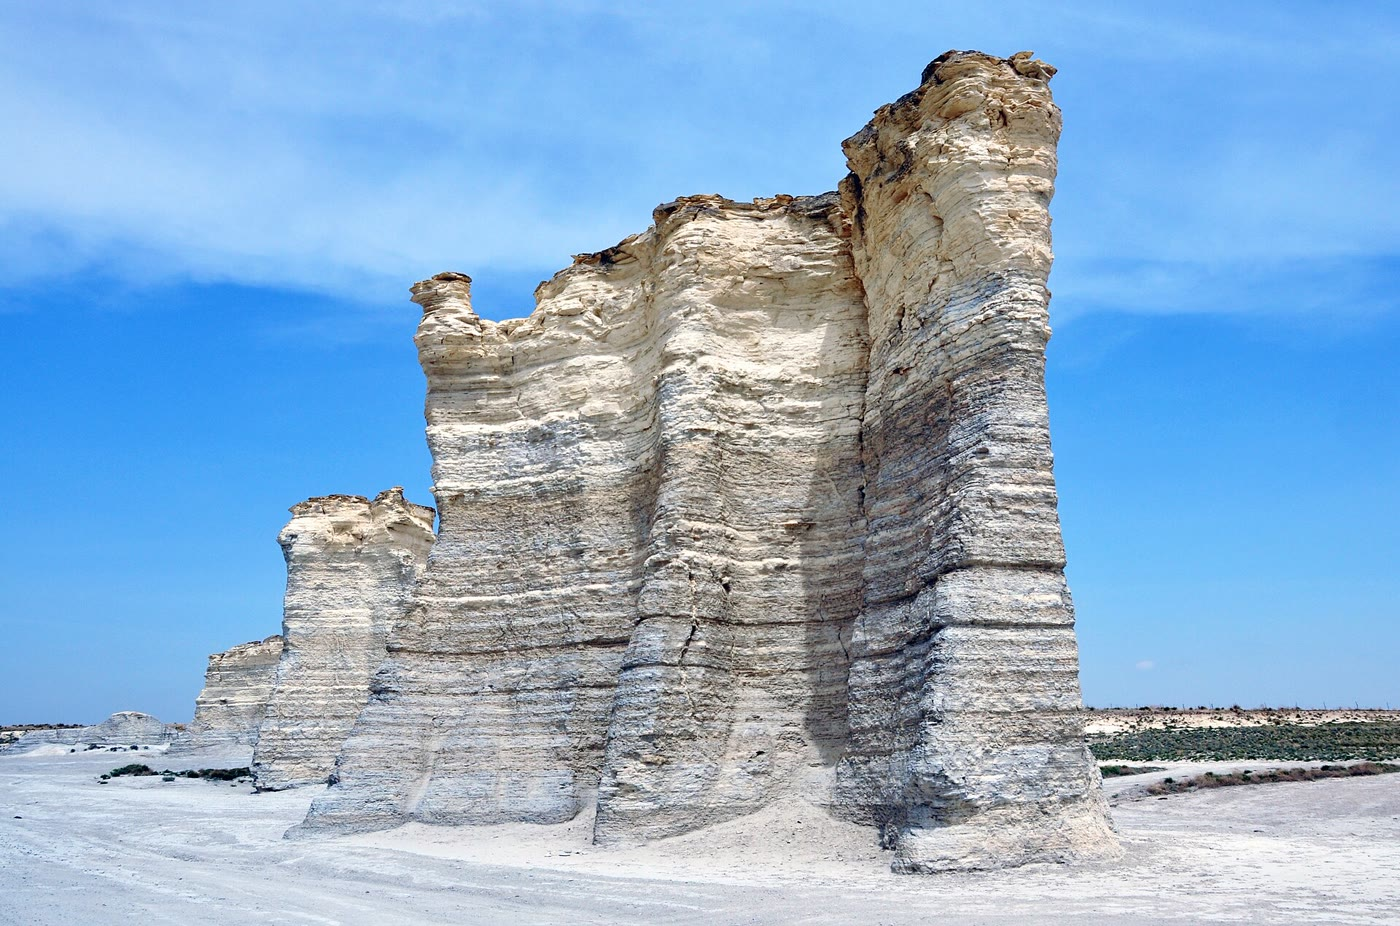
\includegraphics[width=0.66\linewidth]{images/book4/b2-19-monument-rocks.jpg}
\par\smallskip{\small صخور مونيومنت، غرب كانساس: أعمدة من الطباشير، وهو وحل بحر داخلي من
الطباشيري عمره نحو 80 مليون سنة، ترسّب بمعدّل نحو \qty{0.036}{mm} في السنة. الصورة:
\mbox{\textdir TLT James St.~John, CC~BY~2.0 (Wikimedia Commons)}.}
\end{omfigure}
% ledger: kgs:monument-rocks, kgs:chalk

\begin{definition}[البحر فوق القارّي]\label{def:b2:phanerozoic-earth:epeiric}
\emph{البحر فوق القارّي}\index{البحر فوق القارّي} بحر ضحل منتشر فوق داخل
قارّة، على قشرة قارّية، بعيدًا عن الهامش القارّي.
\end{definition}

يبلغ البحر هذه الدواخل بتحريك شاطئه، والصخور تسجّل تلك الحركة.

\begin{definition}[التجاوز البحري؛ الانحسار البحري]\label{def:b2:phanerozoic-earth:transgression}
\emph{التجاوز البحري}\index{التجاوز البحري} انتقال خطّ الشاطئ نحو اليابسة،
ينتشر به البحر فوق الأرض؛ و\emph{الانحسار البحري}\index{الانحسار البحري} انتقاله
نحو البحر، تبرز به الأرض.
\end{definition}

في مقطع رأسي، يكدّس \omterm{def:b2:phanerozoic-earth:transgression}{التجاوز البحري} رواسب المياه الأعمق فوق رواسب المياه الأضحل ---
طين البحر المفتوح فوق رمل الشاطئ --- والانحسار العكس. وكلاهما يتبع مستوى البحر
النسبي، الذي يمزج مستوى البحر العالمي بهبوط المكان أو ارتفاعه وبإمداد
الرواسب: فالدلتا قادرة على دفع شاطئها نحو البحر بينما يرتفع البحر، إن غُذّيت بسرعة
كافية. ولقراءة مستوى البحر العالمي من التجاوزات، يجب على الجيولوجي أن يجد الإشارة نفسها
في عدّة قارّات، أو أن يزيل الهبوط \omterm{def:b2:basins-compared:backstripping}{بالتجريد العكسي}، كما في
\cref{ch:b2:basins-compared}.
% ledger: miller20:rsl

\subsection*{المنحنى الطويل الأمد}

\begin{definition}[دورة مستوى البحر من الرتبة الأولى]\label{def:b2:phanerozoic-earth:first-order}
\emph{دورة مستوى البحر من الرتبة الأولى}\index{دورة مستوى البحر من الرتبة الأولى} هي أبطأ أجزاء
تغيّر مستوى البحر العالمي، على مقاييس زمنية من عشرات إلى مئات ملايين السنين، تحدّدها
تكتونية الأرض الصلبة لا الجليد.
\end{definition}

عبر دهر الحياة الظاهرة يتّخذ منحنى الرتبة الأولى شكل الحرف M: مرتفع في الباليوزوي المبكّر،
ومنخفض بينما تجمّعت بانجيا وبقيت، من الكربوني إلى نهاية الترياسي، ومرتفع
من جديد في الطباشيري، ومنخفض منذ ذلك الحين. وبالاستقراء من أمريكا الشمالية، توحي غمرة
الأوردوفيشي المتأخّر وحدها بارتفاع إضافي من 100 إلى \qty{200}{m}.
وتركب هذا المنحنى تغيّرات أسرع: فالتي يحرّكها الجليد تُسجَّل على مقاييس زمنية من $10^4$ إلى
$10^6$ سنة، والصفيحة الجليدية القطبية الجنوبية، منذ نحو \qty{33.5}{Ma}، حرّكت البحر بمقدار 50 إلى
\qty{60}{m}.
% ledger: th23:flooding, miller11:greenhouse, miller05:abstract

\begin{omfigure}
\centering
% figdata/bachelor-2/phanerozoic.py parts sealevel-haq, sealevel-haqlt, sealevel-kominz, sealevel-kominzlt
\begin{tikzpicture}
\begin{axis}[width=0.92\linewidth, height=6.2cm, x dir=reverse, xmin=0, xmax=252,
  ymin=-130, ymax=280, xlabel={العمر \babelsublr{(\unit{Ma})}}, ylabel={مستوى البحر فوق مستوى اليوم \babelsublr{(\unit{m})}},
  xtick={0,50,...,250}, ytick={-100,-50,...,250}, xtick pos=bottom, ytick pos=left,
  tick label style={font=\scriptsize}, label style={font=\small},
  legend style={at={(0.5,1.04)}, anchor=south, draw=none, font=\scriptsize, legend columns=2,
  /tikz/every even column/.append style={column sep=8pt}}]
\addplot[black!30, line width=0.3pt] table[x=age_ma, y=sl_m]
  {figdata/out/bachelor-2-phanerozoic-sealevel-haq.dat};
\addlegendentry{\foreignlanguage{arabic}{هاك وزملاؤه (1987)}}
\addplot[omThm, line width=0.3pt] table[x=age_ma, y=sl_m]
  {figdata/out/bachelor-2-phanerozoic-sealevel-kominz.dat};
\addlegendentry{\foreignlanguage{arabic}{نيوجيرسي، بالتجريد العكسي}}
\addplot[black, line width=1.2pt] table[x=age_ma, y=sl_m]
  {figdata/out/bachelor-2-phanerozoic-sealevel-haqlt.dat};
\addlegendentry{\foreignlanguage{arabic}{هاك، متوسط \mbox{\textdir TLT 10 Myr}}}
\addplot[omThm!70!black, line width=1.2pt] table[x=age_ma, y=sl_m]
  {figdata/out/bachelor-2-phanerozoic-sealevel-kominzlt.dat};
\addlegendentry{\foreignlanguage{arabic}{نيوجيرسي، متوسط \mbox{\textdir TLT 10 Myr}}}
\addplot[black!50, line width=0.3pt, forget plot] coordinates {(0,0) (252,0)};
\foreach \a/\b/\c in {251.902/201.4/icsTriassic, 201.4/143.1/icsJurassic,
  143.1/66/icsCretaceous, 66/23.04/icsPaleogene, 23.04/2.58/icsNeogene, 2.58/0/icsQuaternary} {
  \edef\tmp{\noexpand\fill[\c] (axis cs:\a,-130) rectangle (axis cs:\b,-112);}\tmp}
\node[font=\tiny, text=white] at (axis cs:226.7,-121) {الترياسي};
\node[font=\tiny, text=white] at (axis cs:172.3,-121) {الجوراسي};
\node[font=\tiny] at (axis cs:104.6,-121) {الطباشيري};
\node[font=\tiny] at (axis cs:44.5,-121) {الباليوجين};
\node[font=\tiny] at (axis cs:12.8,-121) {نيوج.};
\end{axis}
\end{tikzpicture}
\par\smallskip{\small مستوى البحر العالمي منذ \qty{250}{Ma}، كما جدوله ميلر وزملاؤه
(2005): مخطّط الدورات لهاك وزملائه (1987) المستخلص من طبقية أحواض كثيرة، ومستوى
البحر المستخرج \omterm{def:b2:basins-compared:backstripping}{بالتجريد العكسي} من آبار لبابية في نيوجيرسي، مع تقدير مستويات الانخفاض (كومينز
وزملاؤه 2008). الخطوط السميكة: متوسطات متحرّكة على \qty{10}{Myr}، أي اتجاه الرتبة الأولى. والأعمار على
السلّم الزمني لعام 2012؛ ويُظهر الشريط في الأسفل العصور.}
\end{omfigure}
% ledger: data:b4-sealevel, haq87:charts, kominz08:long-term, ics:base.Triassic, ics:base.Jurassic, ics:base.Cretaceous, ics:base.Paleogene, ics:base.Neogene, ics:base.Quaternary, ics:colour.Triassic, ics:colour.Jurassic, ics:colour.Cretaceous, ics:colour.Paleogene, ics:colour.Neogene, ics:colour.Quaternary

يتّفق المنحنيان أعلاه على الشكل ويختلفان في الحجم. فمخطّط الدورات، المبني على
تكدّس الرواسب في أحواض كثيرة، يضع مستوى البحر الطويل الأمد في منتصف الطباشيري
على نحو \qty{233}{m} فوق مستوى اليوم؛ أمّا آبار نيوجيرسي، المجرّدة عكسيًا واحدة بعد أخرى، فتعطي نحو
\qty{70}{m} في الطباشيري المتأخّر وحدًّا أقصى قرب \qty{110}{m} في الإيوسين. ويخلص ميلر
وزملاؤه إلى أن ذروة الطباشيري الطويلة الأمد كانت $100 \pm \qty{50}{m}$، وأن
مخطّطات الدورات، المصيبة في توقيت الانخفاضات، تبالغ في سعاتها. وحتى نيوجيرسي
ليست مقياسًا كاملًا: فبحرها في الطباشيري المتأخّر أخفض بمقدار 100 إلى \qty{150}{m} مما يتنبّأ به حجم
أحواض المحيطات، وهي فجوة قد يفسّرها هبوط المنطقة فوق صفيحة فارالون
المندسّة --- أي التضاريس الديناميكية.
% ledger: data:b4-sealevel, miller05:abstract, kominz08:long-term, miller20:epr

\subsection*{لماذا يتحرّك البحر: الظهرات}

ما الذي يرفع البحر مئة متر طوال عشرات ملايين السنين؟ ليس الجليد: فقد كان الطباشيري
عالمًا دافئًا لا يحمل إلا صفائح جليدية صغيرة قصيرة العمر على الأكثر. والجواب الأرجح هو حجم
الظهرات المحيطية. فقاع المحيط الفتيّ حارّ ومرتفع؛ وكلّما أسرعت الصفائح في الانتشار، كان
القاع أفتى في المتوسط، وكانت أحواض المحيطات أضحل، وفاض مزيد من الماء على
القارّات.
% ledger: miller11:greenhouse, th23:pitman

\begin{proposition}[مستوى البحر ومعدّل الانتشار]\label{prop:b2:phanerozoic-earth:ridge}
ليُصنع قاع محيط مساحته $A_{\text{f}}$ عند ظهرات طولها الكلّي $L$ بمعدّل الانتشار
الكامل $u$، وليُستهلك عند العمر $\tau = A_{\text{f}}/(Lu)$، وكلّ عمر بين 0
و$\tau$ يغطّي المساحة نفسها. وليتبع عمقه القانون $d(t) = d_{\text{r}} + c\sqrt t$.
\begin{enumerate}
  \item متوسط عمق القاع هو $\bar d = d_{\text{r}} + \tfrac23 c\sqrt\tau$.
  \item إذا صار معدّل الانتشار $fu$، مع بقاء $A_{\text{f}}$ و$L$ دون تغيّر، نقص متوسط
        العمق بمقدار $\Delta\bar d = \tfrac23 c\sqrt\tau\,\bigl(1 - f^{-1/2}\bigr)$.
  \item إذا هبط القاع هبوطًا أيزوستاتيًا تحت الماء المضاف، ولم ينتشر البحر
        فوق اليابسة، ارتفع مستوى البحر فوق محيط مساحته $A_{\text{o}}$ بمقدار
        \[
        \Delta s = \frac{\rho_{\text{m}} - \rho_{\text{w}}}{\rho_{\text{m}}}\,
        \frac{A_{\text{f}}}{A_{\text{o}}}\,\Delta\bar d ,
        \]
        حيث $\rho_{\text{m}}$ كثافة الوشاح و$\rho_{\text{w}}$ كثافة ماء البحر.
\end{enumerate}
\end{proposition}

\begin{proof}
(1) تصنع الظهرات قاعًا جديدًا بالمعدّل $Lu$ (مساحة لكل وحدة زمن)، وكلّ شريط من القاع يعيش
الزمن $\tau$؛ وفي حالة مستقرّة تكون مساحة القاع الذي يقع عمره بين $t$ و$t + \mathrm{d}t$
هي $Lu\,\mathrm{d}t$ لكل $t < \tau$، فتكون المساحة الكلّية $Lu\tau = A_{\text{f}}$
والأعمار موزّعة بانتظام. ومتوسط العمق هو
$\frac1\tau\int_0^\tau (d_{\text{r}} + c\sqrt t)\,\mathrm{d}t = d_{\text{r}} + \frac{c}{\tau}
\cdot\frac23\tau^{3/2}$. (2) مع المعدّل $fu$ يصير $\tau$ مساويًا $\tau/f$،
و$\sqrt{\tau/f} = f^{-1/2}\sqrt\tau$. (3) تفقد الأحواض الحجم $\Delta V = A_{\text{f}}
\Delta\bar d$. ليرتفع سطح البحر بمقدار $\Delta s$ بالنسبة إلى القارّات، وليهبط القاع
بمقدار $y$ تحت الماء الإضافي. فعمود الماء الإضافي، الذي سمكه $\Delta s + y$، يحلّ محلّ
سمك $y$ من الوشاح في التوازن الأيزوستاتي: $\rho_{\text{w}}(\Delta s + y) =
\rho_{\text{m}} y$، فيكون $y = \rho_{\text{w}}\Delta s/(\rho_{\text{m}} - \rho_{\text{w}})$
و$\Delta s + y = \Delta s\,\rho_{\text{m}}/(\rho_{\text{m}} - \rho_{\text{w}})$. والحجم
محفوظ: $A_{\text{o}}(\Delta s + y) = \Delta V$، ومنه النتيجة.
\end{proof}

القاع الحقيقي ليس بهذا الترتيب. فأعماره ليست موزّعة بانتظام: القاع الفتيّ هو الأوفر،
والمساحة تتناقص مع العمر، كما تُظهر اللوحة اليسرى أدناه. كما أن قانون الجذر التربيعي لا ينطبق على
القاع القديم، الذي يستوي قرب \qty{6.4}{km}؛ فالقانون الأسّي الذي وفّقه بارسونز وسكليتر
على القاع القديم، قانون الصفيحة، يتولّى الأمر بعد نحو \qty{26}{Myr}، حيث يلتقي
القانونان. والقضيّة تقدير أوّل، ويبيّن الشكل
كم يغيّره القانون الثاني.
% ledger: ps77:depth-age, data:b4-ridge

\begin{omfigure}
\centering
% figdata/bachelor-2/phanerozoic.py parts agehist and ridge
\begin{tikzpicture}
\begin{groupplot}[group style={group size=2 by 1, horizontal sep=1.6cm},
  width=0.5\linewidth, height=5.6cm, tick label style={font=\scriptsize},
  label style={font=\small}, xtick pos=bottom, ytick pos=left]
\nextgroupplot[xmin=0, xmax=200, ymin=0, ymax=34, xlabel={عمر القاع \babelsublr{(\unit{Myr})}},
  ylabel={المساحة لكل \qty{10}{Myr} \babelsublr{(\unit{\mega km^2})}},
  legend style={at={(0.5,1.04)}, anchor=south, draw=none, font=\scriptsize}]
\addplot[ybar interval, area legend, fill=omSea!80!black, draw=black!50, line width=0.2pt]
  table[x expr=\thisrow{age}-5, y=area_Mkm2] {figdata/out/bachelor-2-phanerozoic-agehist.dat};
\addlegendentry{شبكة الأعمار}
\addplot[const plot mark mid, black, dashed, line width=0.9pt]
  table[x=age, y=uniform_Mkm2] {figdata/out/bachelor-2-phanerozoic-agehist.dat};
\addlegendentry{\foreignlanguage{arabic}{أعمار منتظمة حتى \mbox{\textdir TLT \qty{128.4}{Myr}}}}
\nextgroupplot[xmin=1, xmax=3, ymin=0, ymax=650, xlabel={معدّل الانتشار / معدّل اليوم، $f$},
  ylabel={ارتفاع مستوى البحر $\Delta s$ \babelsublr{(\unit{m})}},
  legend style={at={(0.5,1.04)}, anchor=south, draw=none, font=\scriptsize, legend columns=2}]
\fill[omThm!15] (axis cs:1,50) rectangle (axis cs:3,150);
\addplot[black, line width=1pt] table[x=f, y=ds_hs] {figdata/out/bachelor-2-phanerozoic-ridge.dat};
\addlegendentry{\foreignlanguage{arabic}{قانون $\sqrt t$}}
\addplot[blue!70!black, dashed, line width=1pt] table[x=f, y=ds_plate]
  {figdata/out/bachelor-2-phanerozoic-ridge.dat};
\addlegendentry{قانون الصفيحة}
\node[font=\scriptsize, anchor=west] at (axis cs:1.6,100) {$100 \pm \qty{50}{m}$};
\end{groupplot}
\end{tikzpicture}
\par\smallskip{\small يسارًا: مساحة قاع المحيط الحالي في فئات عمرية عرضها \qty{10}{Myr}، من شبكة الأعمار
لسيتون وزملائه (2020) بدقّة درجة واحدة (\qty{293}{\mega km^2} في المجموع)، مقابل
التوزيع المنتظم في \cref{prop:b2:phanerozoic-earth:ridge} بالمساحة نفسها والعمر المتوسط نفسه. يمينًا:
ارتفاع مستوى البحر حين يُضرب معدّل الانتشار في $f$، من القضيّة مع
قانون الجذر التربيعي ومع قانون الصفيحة، انطلاقًا من التوزيع المنتظم حتى \qty{128.4}{Myr}؛
والنطاق هو ذروة الطباشيري الطويلة الأمد التي قدّرها ميلر وزملاؤه (2005).}
\end{omfigure}
% ledger: data:b4-ridge, data:b2-seafloor-age, seton:mean-age, ps77:depth-age, miller05:abstract, charette:ocean-volume, katz03:thermo, noaa:seawater-1025

\begin{example}[ضعف السرعة]\label{ex:b2:phanerozoic-earth:doubling}
خذ قاع اليوم: عمره المتوسط \qty{64.2}{Myr}، فيكون $\tau = \qty{128.4}{Myr}$ في النموذج المنتظم؛
و$d_{\text{r}} = \qty{2500}{m}$، و$c = \qty{350}{m.Myr^{-1/2}}$. ومتوسط العمق $2500 + \tfrac23
\times 350 \times \sqrt{128.4} = \qty{5144}{m}$. ومضاعفة المعدّل تنصّف $\tau$، فيصير متوسط
العمق $2500 + \tfrac23 \times 350 \times \sqrt{64.2} = \qty{4370}{m}$: فيرتفع القاع بمقدار
\qty{774}{m} في المتوسط. ومع $A_{\text{f}}/A_{\text{o}} = 293/362 = 0.8094$
و$(\rho_{\text{m}} - \rho_{\text{w}})/\rho_{\text{m}} = (3300 - 1025)/3300 = 0.689$، يرتفع البحر
بمقدار $0.689 \times 0.8094 \times 774 = \qty{432}{m}$؛ ومع قانون الصفيحة، \qty{368}{m}. وكلاهما
نحو أربعة أضعاف ذروة الطباشيري الطويلة الأمد. وبالقراءة المعاكسة، تقول اللوحة اليمنى إن
معدّل انتشار أعلى من معدّل اليوم بنسبة 15 إلى \qty{20}{\percent} فقط يكفي لرفع البحر \qty{100}{m} --- ولهذا
يخلص ميلر وزملاؤه إلى أن القشرة المحيطية صُنعت في الطباشيري ببطء أكبر بكثير
مما استُنتج يومًا.
\end{example}
% ledger: seton:mean-age, ps77:depth-age, data:b4-ridge, charette:ocean-volume, katz03:thermo, noaa:seawater-1025, miller05:abstract
% values (phanerozoic.py numbers): dbar_hs 5144, dbar_hs_half 4369.6, rise2_hs 432.5, rise2_pl 368.4, f_for_100_hs 1.151

والنموذج أعمق أيضًا مما ينبغي: فمتوسط عمقه، \qty{5144}{m}، يتجاوز متوسط العمق المقيس
للقاع المؤرَّخ، \qty{4265}{m}، جزئيًا لأن قانون الجذر التربيعي يبالغ في القاع القديم،
وجزئيًا لأن القاع الحقيقي يحمل رواسب وجبالًا بحرية وهضابًا يُغفلها القانون. وليس الانتشار
الرافعة الوحيدة. فالظهرات توازنها الخنادق: إذا ارتفع قاع المحيط في مكان، فلا بدّ أن تذهب الكتلة
إلى مكان ما، والقارّة الهابطة فوق كتلة مندسّة --- أي التضاريس الديناميكية --- تُدخل البحر
محلّيًا. ويرى تاسيسترو-هارت وماكدونالد أن غمرات أمريكا الشمالية تتبع الكتل المندسّة
تحت القارّة، وأن مستوى البحر العالمي يتوقّف على مقدار الاندساس الذي يحدث تحت
القارّات لا تحت المحيطات.
% ledger: data:b4-floor-depth, th23:pitman, th23:flooding, kominz08:long-term

\section{غمر القارّات}\label{sec:b2:phanerozoic-earth:flooding}

كم من اليابسة يُغرقه ارتفاع البحر يتوقّف على شكل سطح الأرض، الذي يلخّصه
المنحنى الهيبسومتري في مجلد السنة الأولى: كسر السطح القائم فوق
كلّ ارتفاع (الشكل أدناه، يسارًا). والقارّات مسطّحة القمم. فعلى الشبكة ذات الدرجة الواحدة من
ETOPO1، \qty{29.0}{\percent} من السطح يابسة و\qty{34.3}{\percent} فوق
\qty{-200}{m}: فالأرصفة، المغمورة أصلًا، تصنع الفرق. ومعظم اليابسة منخفض، لذا فإن
ارتفاعًا متواضعًا يغمر قدرًا كبيرًا منها.
% ledger: data:b4-hyps, data:etopo1

\begin{proposition}[غمر اليابسة]\label{prop:b2:phanerozoic-earth:flooding}
لتكن $A_{\text{o}}$ مساحة البحر اليوم و$a(z)$ مساحة اليابسة الأخفض من $z$ فوق
مستوى البحر الحالي. فحجم $V$ من الماء يُضاف إلى البحر يرفع مستواه بالارتفاع $s$
الذي يحقّق
\[
V = \int_0^s \bigl(A_{\text{o}} + a(z)\bigr)\,\mathrm{d}z ,
\]
ويغمر مساحة اليابسة $a(s)$. وبما أن $a \ge 0$، فالارتفاع لا يتجاوز $V/A_{\text{o}}$.
\end{proposition}

\begin{proof}
حين يكون البحر عند $z$ فإنه يغطّي $A_{\text{o}} + a(z)$؛ ورفعه بمقدار $\mathrm{d}z$ يتطلّب
الحجم $\bigl(A_{\text{o}} + a(z)\bigr)\mathrm{d}z$. والجمع من 0 إلى $s$ يعطي $V$.
والمُكامَل لا يقلّ عن $A_{\text{o}}$، فيكون $V \ge A_{\text{o}}s$.
\end{proof}

\begin{omfigure}
\centering
% figdata/bachelor-2/phanerozoic.py parts hyps and flood
\begin{tikzpicture}
\begin{groupplot}[group style={group size=2 by 1, horizontal sep=1.6cm},
  width=0.46\linewidth, height=5.6cm, tick label style={font=\scriptsize},
  label style={font=\small}, xtick pos=bottom, ytick pos=left]
\nextgroupplot[xmin=0, xmax=100, ymin=-9500, ymax=6500,
  xlabel={النسبة المئوية من السطح فوق $z$}, ylabel={الارتفاع $z$ \babelsublr{(\unit{m})}},
  scaled y ticks=false, yticklabel style={/pgf/number format/1000 sep={\,}}]
\addplot[omThm, line width=1pt] table[x=pct, y=z] {figdata/out/bachelor-2-phanerozoic-hyps.dat};
\addplot[black!50, line width=0.3pt] coordinates {(0,0) (100,0)};
\node[font=\scriptsize, anchor=south west] at (axis cs:30,100) {\foreignlanguage{arabic}{اليابسة \mbox{\textdir TLT \qty{29.0}{\percent}}}};
\node[font=\scriptsize] at (axis cs:45,-7000) {قاع المحيط};
\nextgroupplot[xmin=0, xmax=1000, ymin=0, ymax=80, xlabel={ارتفاع مستوى البحر $h$ \babelsublr{(\unit{m})}},
  ylabel={اليابسة المغمورة \babelsublr{(\unit{\percent})}}]
\addplot[omThm, line width=1pt] table[x=h, y=flooded_pct]
  {figdata/out/bachelor-2-phanerozoic-flood.dat};
\addplot[black, dashed, line width=0.5pt] coordinates {(100,0) (100,14.9) (0,14.9)};
\addplot[black, dashed, line width=0.5pt] coordinates {(432,0) (432,50.6) (0,50.6)};
\end{groupplot}
\end{tikzpicture}
\par\smallskip{\small يسارًا: المنحنى الهيبسومتري للأرض من شبكة ETOPO1 ذات الدرجة الواحدة.
يمينًا: النسبة المئوية من يابسة اليوم الواقعة تحت كلّ ارتفاع فوق مستوى البحر، أي اليابسة التي يغمرها ارتفاع $h$
لو لم يتحرّك شيء آخر؛ وتُعلّم الخطوط المتقطّعة \qty{100}{m} و\qty{432}{m}. وأخذ المتوسط على
خلايا من درجة واحدة يملّس التضاريس، فهذه تقديرات أولى.}
\end{omfigure}
% ledger: data:b4-hyps, data:etopo1

تعطي اللوحة اليمنى الجواب فورًا. فارتفاع قدره \qty{100}{m} يُغرق نحو
\qty{15}{\percent} من يابسة اليوم؛ و\qty{432}{m} الناتجة عن مضاعفة معدّل الانتشار تُغرق
نصفها. وبحر كهذا ينتشر فوق اليابسة التي يغمرها، فيكون الارتفاع نفسه أصغر من حدّ
القضيّة $V/A_{\text{o}}$، بنحو العُشر لارتفاع من بضع مئات من الأمتار (مسألة نهاية
الأسبوع). أمّا بحار كانساس الطباشيرية فاحتاجت إلى أقلّ من ذلك بكثير: فداخل القارّة كثيرًا ما يكون
منخفضًا، وقد يهبط أيضًا فوق كتلة مندسّة.
% ledger: data:b4-hyps
% values (phanerozoic.py numbers): flood_100 14.9, flood_rise2 50.8, level_rise2_spread 390.7

\section{الأحزمة الجبلية لدهر الحياة الظاهرة}\label{sec:b2:phanerozoic-earth:orogens}

تنتهي كلّ \omterm{def:b2:wilson-cycle:wilson}{دورة ويلسون} في \cref{ch:b2:wilson-cycle} بحزام جبلي، وأحزمة دهر الحياة الظاهرة
تُعلّم صنع بانجيا وتفكّكها. ويجمع الجدول تلك التي صادفناها في هذا المجلد.

\begin{center}
\small
\begin{tabular}{>{\raggedright\arraybackslash}p{0.15\linewidth}>{\raggedright\arraybackslash}p{0.22\linewidth}>{\raggedright\arraybackslash}p{0.22\linewidth}>{\raggedright\arraybackslash}p{0.29\linewidth}}
\hline
الأوروجينيا & الزمن & المحيط الذي أُغلق & ما التقى \\
\hline
الكاليدونية & من نحو 540 إلى \qty{400}{Ma}؛ والتصادم الرئيسي من 425 إلى \qty{400}{Ma} & يابيتوس & لورنتيا وبالتيكا
وأفالونيا، مكوّنةً لوروسيا \\
الفارسكية--الأبالاشية & منذ نحو \qty{550}{Ma}؛ والتصادم الأخير من الكربوني المتأخّر إلى البرمي & الريئيك &
غوندوانا وأراضيها المنفصلة مع لوروسيا، مكوّنةً بانجيا \\
الألبية & الطباشيري (الذروة قرب \qty{100}{Ma}) والسينوزوي & تيثيس الألبي & أبوليا وأوروبا \\
الهيمالايا & من نحو 60 إلى \qty{54}{Ma} (موضع جدل) حتى اليوم & المحيط شمال الهند & الهند وآسيا \\
الأنديزية & لا تزال نشطة؛ تقصير منذ الأوليغوسين & لا يوجد: صفيحة محيطية تندسّ & صفيحة
نازكا تحت أمريكا الجنوبية \\
\hline
\end{tabular}
\end{center}
% ledger: mckerrow00:caledonian, schiffer20:caledonides, schiffer20:variscan, faure24:variscan, usgs:alleghanian-age, schmid04:two-orogenies, najman21:collision-age, gerbault05:andes, nance22:supercontinents

خاط الحزامان الأوّلان بانجيا، وأغلق الحزام الفارسكي آخر محيط بين غوندوانا
ولوروسيا؛ ونمت الأحزمة الثلاثة الأخيرة بينما تباعدت قطع بانجيا واستُهلكت المحيطات بينها.
ومستوى البحر المنخفض في الباليوزوي المتأخّر والترياسي ينتمي إلى هذه
القارّة العظمى، والبحر المرتفع في الطباشيري إلى تفكّكها، بظهراتها الجديدة وقاعها
الفتيّ.
% ledger: schiffer20:variscan, th23:flooding, nance22:supercontinents

\section{أزمات الحياة}\label{sec:b2:phanerozoic-earth:extinctions}

\subsection*{الخمسة الكبرى}

تصف مجلدات الأحياء الانقراضات الجماعية؛ ويقيسها الجيولوجيون في الصخور ويبحثون عن
أسبابها. وخمسة منها تبرز في سجلّ الحيوانات البحرية، «الخمسة الكبرى»: في نهاية
الأوردوفيشي، نحو \qty{444}{Ma}؛ وفي الديفوني المتأخّر، \qty{372}{Ma}؛ وفي نهاية البرمي،
\qty{251.9}{Ma}؛ وفي نهاية الترياسي، \qty{201.4}{Ma}؛ وفي نهاية الطباشيري،
\qty{66}{Ma}. وأزال كلّ منها بين نحو خُمسَي الأجناس وثلثيها من الحيوانات
البحرية في جداول سيبكوسكي. وكانت أزمة نهاية البرمي الأكبر: \qty{56}{\percent} من
الأجناس بأدقّ تحليل زمني، ونحو \qty{81}{\percent} من الأنواع البحرية --- لا
\qty{96}{\percent} التي كثيرًا ما تُذكر، والتي خلطت بين أزمتين منفصلتين.
% ledger: kaiho22:table, marshall23:big-five, stanley16:permian

\begin{history}[الخمسة الكبرى، بعد أربعين عامًا]
في عام 1982 عدّ د.~م.~روب وج.~ج.~سيبكوسكي فصائل الحيوانات البحرية التي اختفت
في كلّ طابق من 76 طابقًا من دهر الحياة الظاهرة. فبرزت أربع نقاط فوق حدّ الثقة 99 في المئة
لاتجاههما --- آخر طابق من الأوردوفيشي، وآخر طابقين من البرمي وآخر طابق من
الطباشيري --- وبرزت نهاية الترياسي ونهاية الديفوني فوق حدّ 95 في المئة:
تلك هي الخمسة الكبرى. وبعد أربعين عامًا تبقى الخمسة أكبر الأزمات منذ أوائل
الأوردوفيشي، لكنها مع بيانات أفضل لم تعد تنفصل عن متّصل من معدّلات
الانقراض، بل كانت لبعض فترات الكمبري معدّلات أعلى. وكان التحليل الزمني لروب وسيبكوسكي
\qty{7.4}{Myr}، أي متوسط طول الطابق آنذاك؛ وكانت بعض الأزمات مفاجئة، ودام غيرها
مئات آلاف السنين أو أكثر.
\end{history}
% ledger: marshall23:big-five, marshall23:resolution

\begin{omfigure}
\centering
% figdata/bachelor-2/phanerozoic.py parts ext, lip, oae
\begin{tikzpicture}
\begin{axis}[width=0.95\linewidth, height=6.4cm, x dir=reverse, xmin=0, xmax=541,
  ymin=-34, ymax=80, xlabel={العمر \babelsublr{(\unit{Ma})}}, ylabel={الأجناس البحرية المفقودة \babelsublr{(\unit{\percent})}},
  xtick={0,100,...,500}, ytick={0,20,...,80}, xtick pos=bottom, ytick pos=left,
  tick label style={font=\scriptsize}, label style={font=\small}, clip=false]
\addplot[ybar, bar width=5pt, fill=omThm!70, draw=black!60]
  table[x=age, y=value] {figdata/out/bachelor-2-phanerozoic-ext.dat};
\node[font=\tiny, anchor=south] at (axis cs:444,52) {نهاية الأوردوفيشي}; \node[font=\tiny, anchor=south] at (axis cs:372,41) {الديفوني المتأخّر}; \node[font=\tiny, anchor=south] at (axis cs:251.9,66) {نهاية البرمي}; \node[font=\tiny, anchor=south] at (axis cs:201.4,46) {نهاية الترياسي}; \node[font=\tiny, anchor=south] at (axis cs:66,45) {نهاية الطباشيري};
\addplot[only marks, mark=triangle*, mark size=2.6pt, red!70!black]
  table[x=age, y expr=-6] {figdata/out/bachelor-2-phanerozoic-lip.dat};
\addplot[only marks, mark=diamond*, mark size=2.6pt, blue!70!black]
  table[x=age, y expr=-13] {figdata/out/bachelor-2-phanerozoic-oae.dat};
\addplot[only marks, mark=star, mark size=4pt, line width=1pt, black] coordinates {(66,-20)};
\node[font=\tiny, anchor=west, red!70!black] at (axis cs:541,-6) {مقاطعات بركانية كبرى};
\node[font=\tiny, anchor=west, blue!70!black] at (axis cs:541,-13) {أحداث نقص الأكسجين};
\node[font=\tiny, anchor=west] at (axis cs:541,-20) {اصطدام};
\node[font=\tiny, anchor=west] at (axis cs:57,-20) {تشيكشولوب};
\foreach \a/\b/\c in {538.8/486.85/icsCambrian, 486.85/443.1/icsOrdovician,
  443.1/419.62/icsSilurian, 419.62/358.86/icsDevonian, 358.86/298.9/icsCarboniferous,
  298.9/251.902/icsPermian, 251.902/201.4/icsTriassic, 201.4/143.1/icsJurassic,
  143.1/66/icsCretaceous, 66/23.04/icsPaleogene, 23.04/2.58/icsNeogene, 2.58/0/icsQuaternary} {
  \edef\tmp{\noexpand\fill[\c] (axis cs:\a,-34) rectangle (axis cs:\b,-27);}\tmp}
\foreach \x/\t in {512.8/Cm, 465/O, 431.4/S, 389.2/D, 328.9/C, 275.4/P, 226.7/Tr, 172.3/J,
  104.6/K, 44.5/Pg, 12.8/N} {
  \edef\tmp{\noexpand\node[font=\noexpand\tiny] at (axis cs:\x,-30.5) {\t};}\tmp}
\end{axis}
\end{tikzpicture}
\par\smallskip{\small الانقراضات الجماعية الخمسة الكبرى، مع حصّة الأجناس البحرية المفقودة في
جداول سيبكوسكي (كايهو 2022، الجدول~1)، والمقاطعات البركانية الكبرى (المثلّثات، الأعمار المتوسطة
لكورتيو ورين 2003، منذ \qty{259}{Ma})، وأفضل \omterm{def:b2:phanerozoic-earth:oae}{أحداث نقص الأكسجين المحيطي} دراسةً
(المعيّنات) واصطدام تشيكشولوب. ويُظهر الشريط في الأسفل العصور.}
\end{omfigure}
% ledger: kaiho22:table, cr03:table, rigo24:oaes, pickersgill26:chicxulub, ics:base.Cambrian, ics:base.Ordovician, ics:base.Silurian, ics:base.Devonian, ics:base.Carboniferous, ics:base.Permian, ics:base.Triassic, ics:base.Jurassic, ics:base.Cretaceous, ics:base.Paleogene, ics:base.Neogene, ics:base.Quaternary, ics:colour.Cambrian, ics:colour.Ordovician, ics:colour.Silurian, ics:colour.Devonian, ics:colour.Carboniferous, ics:colour.Permian

\subsection*{المقاطعات البركانية الكبرى}

يُظهر الشكل أعلاه النمط الذي أشار إليه مجلد السنة الأولى: فكلّ واحد من أحدث ثلاثة من
الخمسة الكبرى يقترن بمقاطعة بركانية كبرى، مصاطب سيبيريا في نهاية البرمي،
والمقاطعة الصهارية لوسط الأطلسي (CAMP) في نهاية الترياسي، ومصاطب الدكن في
نهاية الطباشيري. والرابط المقترح هو الغاز. فالبازلت الفيضي يثور في نبضات تدوم من بضعة
قرون إلى بضعة آلاف من السنين، تطلق كلّ منها ثاني أكسيد الكربون أسرع مما تستطيع التجوية استعادته؛
وكبريت الثورانات نفسها يبرّد المناخ لفترة وجيزة، أمّا الكربون فيدفّئه لمدّة أطول
بكثير ويحمّض المحيط.
% ledger: cr03:table, cr03:summary, capriolo20:camp-co2

\begin{example}[كربون المقاطعة الوسطى الأطلسية]\label{ex:b2:phanerozoic-earth:camp}
تُظهر فقاعات الغاز في احتواءات المصهور في بازلتات CAMP أن \omterm{def:b2:magma-emplacement:magma}{الصهارة} حملت ما لا يقلّ عن 0.5 إلى
\qty{0.6}{\percent} من ثاني أكسيد الكربون كتليًا. خذ \qty{0.55}{\percent}، وكثافة
\qty{2900}{kg.m^{-3}} وحجمًا قدره \qty{5.5e6}{km^3}، أي الحمم الثائرة مع القواطع والعتبات
والحجرات التي غذّتها. فكتلة \omterm{def:b2:magma-emplacement:magma}{الصهارة} $\num{5.5e6} \times \num{e9} \times 2900 =
\qty{1.6e19}{kg}$، وثاني أكسيد الكربون فيها $\num{1.6e19} \times 0.0055 = \qty{8.8e16}{kg}$، أي نحو
\qty{9e4}{Gt} --- وهو «حتى \qty{e5}{Gt}» عند المؤلّفين. وقد أُطلق على مدى عمر المقاطعة، فلم
يكن كلّه في الهواء دفعة واحدة؛ لكن كلّ نبضة، من رتبة \qty{e5}{km^3} في بضعة
قرون، أطلقت قدر الانبعاثات المتوقّعة للقرن الحادي والعشرين.
\end{example}
% ledger: capriolo20:camp-co2
% values: 5.5e6 km3 x 2900 kg/m3 = 1.595e19 kg; x 0.0055 = 8.77e16 kg

\subsection*{أحداث نقص الأكسجين المحيطي}

ليست كلّ أزمة من الخمسة الكبرى. فعدّة مرّات في الميزوزوي اختفى الأكسجين من
أجزاء واسعة من المحيط.

\begin{definition}[حدث نقص الأكسجين المحيطي]\label{def:b2:phanerozoic-earth:oae}
\emph{حدث نقص الأكسجين المحيطي}\index{حدث نقص الأكسجين المحيطي} (OAE) فترة من
استنزاف واسع للأكسجين في المحيط، يُتعرّف عليها في السجلّ الرسوبي والجيوكيميائي.
\end{definition}

علامته المعتادة طين صفحي أسود: داكن، دقيق التصفّح، بلا جحور، غنيّ بالمادة العضوية
وبالبيريت، وكثيرًا ما يرافقه انزياح في نظائر الكربون وعلامات احترار. وأفضلها دراسةً
حدث التوارسي المبكّر، نحو \qty{183}{Ma}، وحدث الأبتي المبكّر \babelsublr{OAE~1a}، نحو \qty{120}{Ma}،
وحدث الألبي المبكّر \babelsublr{OAE~1b}، نحو \qty{111}{Ma}، والحدث \babelsublr{OAE~2} عند الحدّ بين السينوماني
والتوروني، نحو \qty{94}{Ma}، في أحرّ أجزاء الطباشيري، حين كان البحر
مرتفعًا ارتفاعًا استثنائيًا. ويتزامن عدد منها مع مقاطعة: حدث التوارسي مع بازلتات كارو--فيرار،
و\babelsublr{OAE~1a} مع هضبة أونتونغ جاوة. وكثيرًا ما يُربط \babelsublr{OAE~2} بهضبة الكاريبي، لكن
قمم الزئبق في رواسب نصف الكرة الجنوبي تشير بالأحرى إلى مقاطعة كيرغولن.
% ledger: rigo24:oaes, wt24:oae2, cr03:table

\begin{omfigure}
\centering
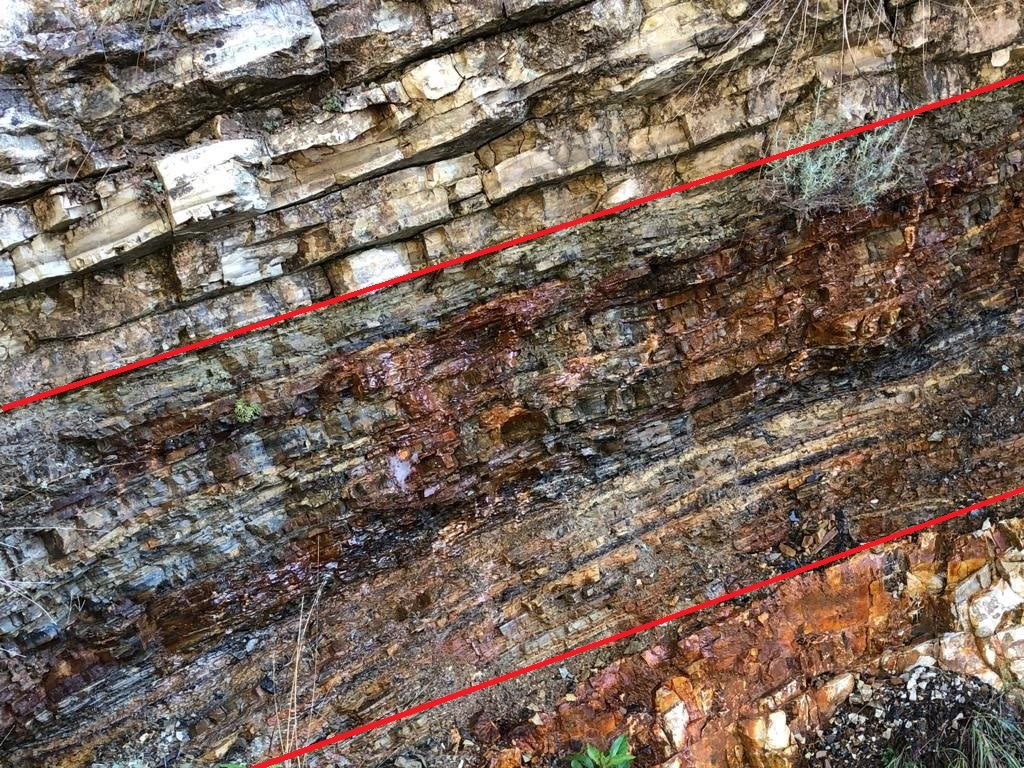
\includegraphics[width=0.66\linewidth]{images/book4/b2-19-bonarelli-level.jpg}
\par\smallskip{\small مستوى بوناريلي، الطين الصفحي الداكن للحدث \babelsublr{OAE~2}، بين أحجار جيرية باهتة؛
والخطّان الأحمران، اللذان رسمهما المصوّر، يُعلّمان قاعدته وقمّته. الصورة:
\mbox{\textdir TLT Picenus, CC~BY-SA~4.0 (Wikimedia Commons)}.}
\end{omfigure}
% ledger: rigo24:oaes

\begin{inthefield}[تسجيل حدث نقص أكسجين]
تسجّل الجيولوجية التي تدرس حدث نقص أكسجين في مقطع من الأحجار الجيرية البحرية العميقة طبقةً بعد طبقة:
السمك، واللون، والتصفّح، والجحور أو غيابها، وعُقد البيريت. وتأخذ العيّنات على فترات
متقاربة منتظمة عبر الفترة الداكنة وأبعد منها بكثير، لمحتوى الكربون العضوي ولنظائر
الكربون في المادة العضوية وفي الكربونات؛ فانزياح النظائر، أكثر من
لون الصخر، هو ما يربط الحدث من حوض إلى آخر. ولأن أدكن
طين صفحي قد يظهر عند مستويات مختلفة في أحواض مختلفة، يُتّخذ منحنى النظائر، لا الطين الصفحي
الأسود، خطًّا زمنيًا.
\end{inthefield}
% ledger: rigo24:oaes, wt24:oae2

\subsection*{تشيكشولوب}

كان لنهاية الطباشيري سبب من الخارج. فقد روى مجلد السنة الأولى كيف قاد إيريديوم
طين الحدّ إلى اصطدام، وكيف ربط التأريخ بالأرغون الحدَّ بفوهة تشيكشولوب.
يبلغ عرض البنية نحو \qty{200}{km} وعمرها \qty{66}{Ma}؛ وغذّت
صخورها الحارّة ماءً دائرًا ثمانية ملايين سنة على الأقلّ بعد ذلك. وتشير نماذج عدم تناظرها
تحت السطح إلى جسم صادم جاء من الشمال الشرقي بزاوية 45 إلى \ang{60} على الأفق،
بسرعة لا تقلّ عن سرعة الإفلات من الأرض، \qty{11.2}{km.s^{-1}}، والأرجح نحو
\qty{20}{km.s^{-1}}. وكانت مصاطب الدكن تثور في الوقت نفسه، قبل الاصطدام
وبعده؛ وقد خلصت مراجعة للأدلّة عام 2010 إلى أن الاصطدام أطلق الانقراض.
% ledger: pickersgill26:chicxulub, collins20:impact, renne:kpg, alvarez:iridium, schulte:kpg, cr03:deccan

\begin{dated}{2026}
الأعمار في هذا الفصل هي أعمار الجدول الكرونوستراتغرافي الدولي في نسخة يونيو
2026، كما في هذه السلسلة كلّها؛ وسجلّات مستوى البحر على السلّم الزمني لعام 2012
في ملفّاتها، وأعمار الانقراضات هي أعمار كايهو (2022). ويُراجَع الجدول كلّما وردت
تواريخ جديدة: فتحقّق من النسخة الحالية قبل الاستشهاد بعمر حدّ.
\end{dated}
% ledger: ics:base.Phanerozoic, data:b4-sealevel, kaiho22:table

\section*{التمارين}\label{sec:b2:phanerozoic-earth:exercises}

معطيات التمارين، ما لم يُذكر غير ذلك: \qty{111.2}{km} لكل درجة عرض؛ وعمق
قاع المحيط $d(t) = 2500 + 350\sqrt t$ (بوحدة \unit{m}، و$t$ بوحدة \unit{Myr})؛ ومساحة المحيط
\qty{362}{\mega km^2}؛ ومساحة قاع المحيط \qty{293}{\mega km^2}؛ وكثافة الوشاح
\qty{3300}{kg.m^{-3}}؛ وماء البحر \qty{1025}{kg.m^{-3}}؛ وكتلة الغلاف الجوي
\qty{5.1e18}{kg}، والكتلتان الموليتان للهواء ولثاني أكسيد الكربون \qty{28.97}{g.mol^{-1}}
و\qty{44.01}{g.mol^{-1}}.
% ledger: earth:Rmean, ps77:depth-age, charette:ocean-volume, data:b4-ridge, katz03:thermo, noaa:seawater-1025, earth:Matm, earth:Mmol, ciaaw:abridged-2024

\begin{exercise}[$\star$]\label{exo:b2:phanerozoic-earth:1}
في نموذج الخرائط، كانت كيب تاون عند \ang{61.9} جنوبًا قبل \qty{300}{Ma} ونيويورك عند
\ang{3.6} جنوبًا؛ وهما اليوم عند \ang{33.9} جنوبًا و\ang{40.7} شمالًا. (أ) أيّ المدن الأربع كانت
على بعد لا يتجاوز \ang{30} من خطّ الاستواء قبل \qty{300}{Ma} (باريس عند \ang{5.1} شمالًا، وسيدني عند
\ang{59.5} جنوبًا)؟ (ب) كم كيلومترًا انتقلت كلّ من كيب تاون ونيويورك شمالًا منذ ذلك الحين؟
(ج) بأيّ معدّلات متوسطة، بالسنتيمتر في السنة؟
\end{exercise}
% ledger: data:b4-palaeopos, geonames4:cities

\begin{exercise}[$\star$]\label{exo:b2:phanerozoic-earth:2}
وقعت الخمسة الكبرى عند 444 و372 و251.9 و201.4 و\qty{66}{Ma}. (أ) أوجد الفترات بين
الأزمات المتعاقبة ومتوسطها. (ب) باستعمال الأعمار المتوسطة للمقاطعات البركانية الكبرى ---
إيميشان 259، وسيبيريا 250، وCAMP 201، وكارو--فيرار 183، والدكن \qty{65.5}{Ma} --- أيّ
الخمس يقع في حدود \qty{2}{Myr} من مقاطعة؟ (ج) هل يجعل متوسط الفترة الأزمات دورية؟
\end{exercise}
% ledger: kaiho22:table, cr03:table

\begin{exercise}[$\star$]\label{exo:b2:phanerozoic-earth:3}
ترسّب طباشير صخور مونيومنت بمعدّل نحو \qty{0.036}{mm} في السنة. (أ) كم استغرق ترسّب
\qty{91}{m} منه؟ (ب) كم مرة أسرع يرتفع البحر اليوم، بمعدّل \qty{3.7}{mm} في
السنة؟ (ج) لماذا يستطيع قاع بحر أن يجمع مطرًا بطيئًا كهذا من الرواسب دون أن يدفنه الطين؟
\end{exercise}
% ledger: kgs:monument-rocks, ipcc:sea-level-obs

\begin{exercise}[$\star$]\label{exo:b2:phanerozoic-earth:4}
في جرف، من الأسفل إلى الأعلى: حجر رملي نهري بجذور، ورمل شاطئ بأصداف، وطين رمادي من البحر
المفتوح، وطباشير؛ ثم يعلو الطباشيرَ رملُ شاطئ من جديد. (أ) أين يسجّل المقطع
تجاوزًا بحريًا، وأين انحسارًا؟ (ب) هل يثبت \omterm{def:b2:phanerozoic-earth:transgression}{التجاوز البحري} أن مستوى البحر العالمي
ارتفع؟ (ج) ما الذي يجعله أكثر إقناعًا؟
\end{exercise}

\begin{exercise}[$\star\star$]\label{exo:b2:phanerozoic-earth:5}
على المنحنى الطويل الأمد لهاك وزملائه، كان مستوى البحر \qty{233}{m} فوق مستوى اليوم عند
\qty{97}{Ma}. (أ) ما المعدّل المتوسط للانخفاض منذ ذلك الحين، بالمتر لكل مليون سنة وبالميكرومتر
في السنة؟ (ب) قارن بارتفاع اليوم البالغ \qty{3.7}{mm} في السنة. (ج) يعطي منحنى نيوجيرسي
المستخرج \omterm{def:b2:basins-compared:backstripping}{بالتجريد العكسي} نحو \qty{70}{m} في الزمن نفسه. بأيّهما تثق في
السعة، ولماذا؟
\end{exercise}
% ledger: data:b4-sealevel, ipcc:sea-level-obs, miller05:abstract, miller20:epr

\begin{exercise}[$\star\star$]\label{exo:b2:phanerozoic-earth:6}
نبضة واحدة من CAMP، نحو \qty{e5}{km^3} من البازلت كثافته \qty{2900}{kg.m^{-3}}،
ثارت في نحو 500 سنة. (أ) مع \qty{0.75}{\percent} من ثاني أكسيد الكربون كتليًا، كم
أطلقت، بالكيلوغرام وبالمول؟ (ب) ما كتلة ثاني أكسيد الكربون التي حملها الهواء عند
\qty{278}{ppm} عام 1750؟ (ج) قارن. (د) كم غلافًا جويًا كهذا كانت المقاطعة كلّها،
\qty{e5}{Gt}، ستوفّر؟
\end{exercise}
% ledger: capriolo20:camp-co2, ipcc:erf-2xco2, earth:Matm, earth:Mmol, ciaaw:abridged-2024

\begin{exercise}[$\star\star$]\label{exo:b2:phanerozoic-earth:7}
اعتبر الجسم الصادم في تشيكشولوب كرة قطرها \qty{10}{km}، كثافتها
\qty{2630}{kg.m^{-3}}. (أ) أوجد كتلته. (ب) أوجد طاقته الحركية عند أدنى سرعة
ممكنة، \qty{11.2}{km.s^{-1}}، وعند \qty{20}{km.s^{-1}}. (ج) تفقد الأرض \qty{47}{TW} من
حرارتها الداخلية عبر سطحها. كم سنة من هذا الفقد تمثّل كلّ طاقة؟
\end{exercise}
% ledger: alvarez:iridium, collins20:impact, b2dd10:half-space

\begin{exercise}[$\star\star$]\label{exo:b2:phanerozoic-earth:8}
(أ) عدّد السمات التي يسجّل بها الطين الصفحي الأسود حدث نقص أكسجين محيطيًا. (ب) قابل كلّ
حدث بمقاطعة من العمر نفسه تقريبًا: التوارسي المبكّر، \qty{183}{Ma}؛ و\babelsublr{OAE~1a}،
\qty{120}{Ma}؛ علمًا بأن كارو--فيرار عند \qty{183}{Ma} وأونتونغ جاوة عند \qty{122}{Ma}. (ج) لماذا لا
يكفي تزامن الأعمار لإثبات أن مقاطعة سبّبت حدثًا؟
\end{exercise}
% ledger: rigo24:oaes, cr03:table

\begin{exercise}[$\star\star$]\label{exo:b2:phanerozoic-earth:9}
في النموذج، كانت باريس عند \ang{60.9} جنوبًا قبل \qty{500}{Ma} وعند \ang{5.1} شمالًا قبل \qty{300}{Ma}.
(أ) أوجد إزاحتها نحو الشمال بالدرجات وبالكيلومترات، والمعدّل المتوسط
بالسنتيمتر في السنة. (ب) قارن بالمعدّل منذ \qty{300}{Ma}
(\cref{ex:b2:phanerozoic-earth:paris}). (ج) لماذا يكون المعدّل حدًّا أدنى؟
\end{exercise}
% ledger: data:b4-palaeopos

\begin{exercise}[$\star\star\star$]\label{exo:b2:phanerozoic-earth:10}
افترض بدلًا من ذلك أن مساحة القاع تتناقص خطّيًا مع العمر، من حدّ أقصى عند العمر 0 إلى الصفر
عند العمر $T$. (أ) بيّن أن العمر المتوسط $T/3$ وأن متوسط $\sqrt t$ هو
$\tfrac{8}{15}\sqrt T$. (ب) مع عمر متوسط قدره \qty{64.2}{Myr}، أوجد $T$ ومتوسط العمق. (ج)
أوجد انخفاض متوسط العمق حين يتضاعف معدّل الانتشار، وقارن بمقدار
\qty{774}{m} في النموذج المنتظم. (د) بيّن أن الانخفاض في النموذجين قريب من $0.93\,c\sqrt{\bar
t}\,(1 - f^{-1/2})$، حيث $\bar t$ العمر المتوسط.
\end{exercise}

\begin{exercise}[$\star\star\star$]\label{exo:b2:phanerozoic-earth:11}
(أ) من \cref{prop:b2:phanerozoic-earth:ridge}، بيّن أن $\Delta s(f) = \Delta s(2)\,(1 -
f^{-1/2})/(1 - 2^{-1/2})$. (ب) مع $\Delta s(2) = \qty{432}{m}$، أوجد مدى $f$ الذي
يعطي ذروة الطباشيري، 50 إلى \qty{150}{m}. (ج) ماذا يفعل معدّل انتشار تباطأ إلى 0.8 من
معدّل اليوم؟ (د) لماذا يكون مستوى البحر الطويل الأمد الذي تحدّده الظهرات إشارةً بطيئة، أيًّا كان تغيّر
المعدّل؟
\end{exercise}
% ledger: data:b4-ridge, miller05:abstract

\begin{exercise}[$\star\star\star$]\label{exo:b2:phanerozoic-earth:12}
افترض أن الأنواع تنقرض بمعدّل ثابت، بحيث يكون كسر الفوج الذي يبقى بعد زمن
$t$ هو $2^{-t/m}$، مع عمر وسيط للنوع $m = \qty{2}{Myr}$. (أ) ما كسر
الفوج الذي يزول بعد \qty{7.4}{Myr}، أي متوسط طول الطابق في تحليل 1982؟ (ب) كم
يستغرق انقراض الخلفية لإزالة \qty{81}{\percent} من الأنواع؟ (ج) دامت أزمة نهاية البرمي
نحو \qty{60}{kyr}. كم كانت أسرع؟ (د) لماذا يطمس التحليل الزمني الخشن
الفرق بين الانقراض الجماعي وانقراض الخلفية؟
\end{exercise}
% ledger: marshall23:resolution, stanley16:permian, burgess:end-permian

\begin{problem}[{مسألة نهاية الأسبوع --- حين كانت الظهرات سريعة}]\label{pb:b2:phanerozoic-earth:1}
تسأل هذه المسألة كم سيرتفع البحر، وكم من اليابسة سيُغرق، لو انتشرت
الظهرات بضعف السرعة. استعمل معطيات التمارين؛ فالعمر المتوسط لقاع المحيط
\qty{64.2}{Myr}، وطول الظهرات الكلّي \qty{65000}{km}، ويحوي محيط اليوم
\qty{1.33e9}{km^3}، وتغطّي اليابسة \qty{148}{\mega km^2}. ويعطي الجدول النسبة المئوية من
يابسة اليوم الواقعة على أقلّ من $h$ فوق مستوى البحر، من شبكة ETOPO1 ذات الدرجة الواحدة.
\begin{center}
\small
\begin{tabular}{lcccccc}
\hline
$h$ \babelsublr{(\unit{m})} & 0 & 100 & 200 & 300 & 400 & 500 \\
اليابسة تحت $h$ \babelsublr{(\unit{\percent})} & 0 & 14.9 & 28.2 & 38.7 & 48.1 & 55.8 \\
\hline
\end{tabular}
\end{center}
افترض، كما في \cref{prop:b2:phanerozoic-earth:ridge}، أن كلّ عمر من أعمار القاع بين 0
والعمر $\tau$ الذي يندسّ عنده يغطّي المساحة نفسها.

\noindent\textbf{الجزء الأول --- قاع المحيط اليوم.}
\begin{enumerate}
  \item أوجد عمق القاع عند الأعمار 0 و25 و64.2 و\qty{100}{Myr}.
  \item أوجد $\tau$ من العمر المتوسط، وعمق أقدم قاع.
  \item أوجد معدّل الانتشار الكامل المتوسط $u = A_{\text{f}}/(L\tau)$، بالكيلومتر لكل مليون
        سنة وبالمليمتر في السنة. هل هو معدّل بطيء أم متوسط أم سريع؟
  \item بيّن أن متوسط عمق القاع هو $2500 + \tfrac23 \times 350\sqrt\tau$،
        واحسبه.
  \item متوسط العمق المقيس للقاع المؤرَّخ \qty{4265}{m}. أعطِ سببين يجعلان
        النموذج أعمق.
  \item ما حجم الماء الذي يقع فوق القاع في النموذج؟ قارن بحجم
        المحيط كلّه.
\end{enumerate}

\noindent\textbf{الجزء الثاني --- ظهرة في مقطع عرضي.}
\begin{enumerate}[resume]
  \item أوجد نصف معدّل الانتشار $v$، مقرّبًا إلى أقرب \qty{0.1}{km.Myr^{-1}}، وعرض
        القاع على كلّ جانب من الظهرة.
  \item ما عمق القاع على بعد \qty{1000}{km} من المحور؟
  \item بيّن أن مساحة المقطع العرضي للظهرة فوق عمق أقدم قاع، باحتساب
        الجانبين كليهما، هي $\tfrac23 v c\,\tau^{3/2}$، واحسبها
        بالكيلومتر المربّع.
  \item أوجد حجم منظومة الظهرات كلّها فوق ذلك العمق.
  \item ما الكسر الذي يمثّله ذلك من حجم المحيط؟
  \item لماذا تقف الظهرة الأسرع انتشارًا أعلى في المتوسط؟
\end{enumerate}

\noindent\textbf{الجزء الثالث --- ضعف السرعة.}
\begin{enumerate}[resume]
  \item يتضاعف معدّل الانتشار مع بقاء مساحة القاع وطول الظهرات. أوجد $\tau$ الجديد
        ومتوسط العمق الجديد.
  \item بكم ينخفض متوسط العمق؟
  \item ما حجم الماء الذي يدفعه القاع خارج الأحواض؟
  \item لو وُزّع على محيط اليوم، فكم يرفع البحر؟
  \item أدخل هبوط القاع تحت الماء الإضافي لتجد الارتفاع $\Delta s$.
  \item كانت ذروة الطباشيري الطويلة الأمد نحو \qty{100}{m}. ما زيادة معدّل الانتشار
        التي تعطي ذلك؟
\end{enumerate}

\noindent\textbf{الجزء الرابع --- البحر فوق اليابسة.}
\begin{enumerate}[resume]
  \item ما مساحة اليابسة التي يغمرها ارتفاع قدره \qty{100}{m}؟
  \item ما المساحة التي يغمرها ارتفاع قدره \qty{432}{m}، بالاستكمال من الجدول؟
  \item لماذا يجب أن يرتفع البحر بأقلّ من \qty{432}{m} متى انتشر فوق اليابسة؟
  \item أوجد الحجم اللازم لرفع البحر بخطوات من \qty{100}{m} حتى \qty{400}{m}،
        بأخذ متوسط المساحة المغمورة على كلّ خطوة (\cref{prop:b2:phanerozoic-earth:flooding}).
        والحجم الذي يجب وضعه هو $\qty{0.432}{km} \times \qty{362}{\mega km^2}$. أين
        يتوقّف البحر؟
  \item ما النسبة المئوية من يابسة اليوم التي يغطّيها عندئذٍ؟
  \item خلاصة: في هذا النموذج، بكم ترفع مضاعفة معدّل الانتشار البحر؟
\end{enumerate}
\end{problem}
% ledger: ps77:depth-age, seton:mean-age, seton:rate-classes, noaa:ridge, charette:ocean-volume, data:b4-ridge, data:b4-floor-depth, katz03:thermo, noaa:seawater-1025, data:b4-hyps, miller05:abstract
